\subsection{UCW10 - Ricerca di un locale tramite nome}
\begin{figure}[!h]
\centering
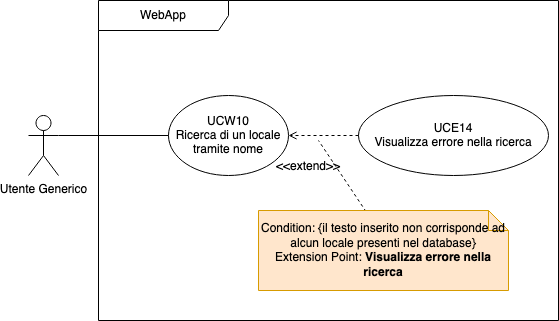
\includegraphics[scale=0.5]{UC_images/UCW10.png} 
\caption{UCW10 - Ricerca di un locale tramite nome}
\end{figure}
\begin{itemize}
    \item \textbf{Descrizione}: L'utente generico effettua la ricerca di un locale tramite il suo nome.
    \item \textbf{Attore primario}: Utente generico.
    \item \textbf{Precondizione}: L'utente si trova all’interno della piattaforma Sweeat.
    \item \textbf{Postcondizione}: Viene visualizzato la lista dei locali ricercati.
    \item \textbf{Scenario principale}: 
    \begin{enumerate}
        \item L’utente va nella barra di ricerca della piattaforma;
        \item L’utente digita il nome del locale da cercare;
        \item L’utente clicca sul bottone di ricerca.
    \end{enumerate}
    \item \textbf{Estensioni}:
    \begin{itemize}
        \item Nel caso in cui l’utente inserisca un testo non corrispondente a nessun locale presente nel database
	\begin{enumerate}  
		\item L’utente va nella barra di ricerca della piattaforma;
        \item L’utente digita il nome del locale da cercare;
        \item L’utente clicca sul bottone di ricerca; 
        \item Viene mostrato un messaggio d'errore, nel caso non sia presente alcun locale simile al locale ricercato(UCE14 §3.28).
    	%Visualizzazione di un messaggio informando che non è presente nessun locale con tale nome e viene suggerita una lista di locali simili a quello ricercato.   
    \end{enumerate}
    \end{itemize}    
\end{itemize}

\subsection{UCW11 - Visualizza informazioni locale}
\begin{figure}[!h]
\centering
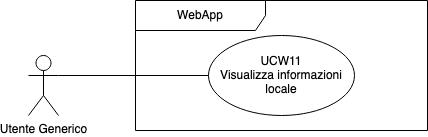
\includegraphics[scale=0.5]{UC_images/UCW11.png} 
\caption{UCW11 - Visualizza informazioni locale}
\end{figure}
\begin{itemize}
    \item \textbf{Descrizione}: L'utente generico visualizza le informazioni di un locale.
    \item \textbf{Attore primario}: Utente generico.
    \item \textbf{Precondizione}: L'utente ha svolto la funzione di ricerca di un locale o sta visualizzando la classifica dei locali.
    \item \textbf{Postcondizione}: Vengono visualizzate le informazioni di base di un locale:
    \begin{enumerate}
        \item Visualizza informazioni generali;
        \item Visualizza punteggio locale;
        \item Visualizza dati estratti;
        \item Visualizza icona preferiti.
        \end{enumerate}
    \begin{figure}[!h]
	\centering
		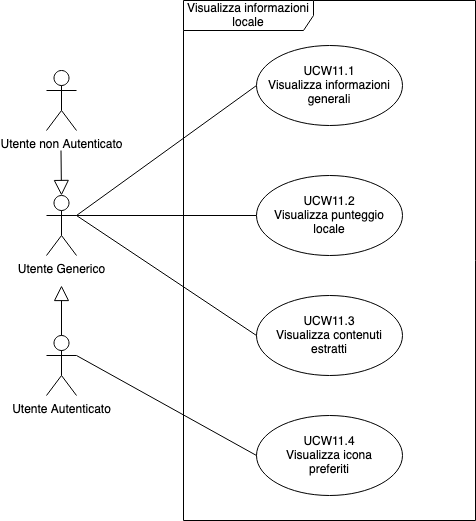
\includegraphics[scale=0.5]{UC_images/UCW11-.png} 
		\caption{Sottocasi UCW11}
	\end{figure}    
    \item \textbf{Scenario principale}: 
    \begin{enumerate}
	\item L'utente visualizza la classifica dei locali presenti nel sistema;
    \item Per ciascun locale, la lista mostrerà alcune informazioni di base.
    \end{enumerate}
\end{itemize}

\subsubsection{UCW11.1 - Visualizza informazioni generali}
\begin{itemize}
    \item \textbf{Descrizione}: L'utente generico visualizza le informazioni di un locale.
    \item \textbf{Attore primario}: Utente generico.
    \item \textbf{Precondizione}: L'utente ha svolto la funzione di ricerca di un locale o sta visualizzando la classifica dei locali.
    \item \textbf{Postcondizione}: Vengono visualizzate le principali informazioni di base di ciascun locale.
	\item \textbf{Sottocasi}:
	\begin{enumerate}
		\item Visualizza nome (UCW11.1.1 \S{});
		\item Visualizza posizione (UCW11.1.2 \S{});
		\item Visualizza categoria (UCW11.1.3 \S{});
		\item Visualizza orari (UCW11.1.4 \S{});
		\item Visualizza numero di telefono (UCW11.1.5 \S{});
		\item Visualizza sito web (UCW11.1.6 \S{}).
	\end{enumerate}
	\begin{figure}[!h]
	\centering
	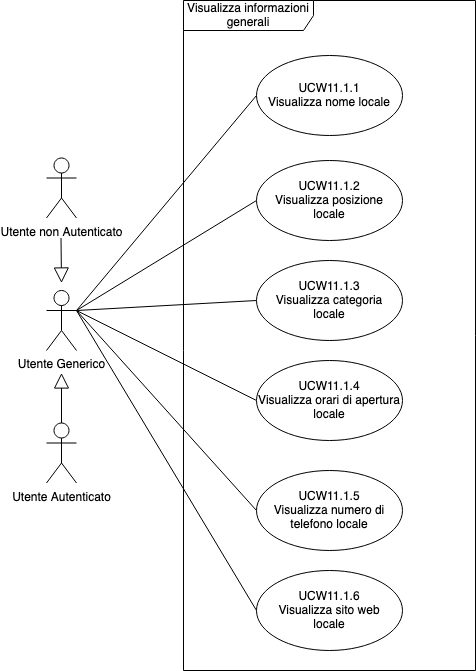
\includegraphics[scale=0.5]{UC_images/UCW11-1.png} 
	\caption{sottocasi UCW11.1}
	\end{figure}
    \item \textbf{Scenario principale}: 
    \begin{enumerate}
	\item L'utente visualizza la classifica dei locali, inseriti sotto forma di lista, presenti nel sistema;
    \item L'utente identifica un locale tra quelli presenti nella lista;
    \item Il sistema mostrerà all'utente le principali informazioni relative al locale scelto.
    \end{enumerate}
\end{itemize}

\subsubsection{UCW11.2 - Visualizza punteggio locale}
\begin{itemize}
    \item \textbf{Descrizione}: L'utente generico visualizza il punteggio di un locale.
    \item \textbf{Attore primario}: Utente generico.
    \item \textbf{Precondizione}: L'utente ha svolto la funzione di ricerca di un locale o sta visualizzando la classifica dei locali.
    \item \textbf{Postcondizione}: Viene visualizzato il punteggio del locale selezionato, calcolato analizzando i contenuti pubblicati sui social.
    \item \textbf{Sottocasi}:
	\begin{enumerate}
		\item Visualizza punteggio totale (UCW11.2.1 \S{});
		\item Visualizza punteggio contenuti multimediali (UCW11.2.2 \S{});
		\item Visualizza punteggio testi (UCW11.2.3 \S{});
		\item Visualizza punteggio emoticon (UCW11.2.4 \S{}).
	\end{enumerate}
    \item \textbf{Scenario principale}: 
    \begin{enumerate}
	\item L'utente visualizza la classifica dei locali, inseriti sotto forma di lista, presenti nel sistema;    
    \item L'utente identifica un locale tra quelli presenti nella lista;
    \item Il sistema mostrerà all'utente la valutazione complessiva del locale scelto.
    \end{enumerate}
\end{itemize}

\subsubsection{UCW11.3 - Visualizza dati estratti}
\begin{itemize}
    \item \textbf{Descrizione}: L'utente generico visualizza le informazioni di un locale.
    \item \textbf{Attore primario}: Utente generico.
    \item \textbf{Precondizione}: L'utente ha svolto la funzione di ricerca di un locale o sta visualizzando la classifica dei locali.
    \item \textbf{Postcondizione}: Vengono visualizzati i dati del locale selezionato estratti dai social.
    \item \textbf{Sottocasi}:
	\begin{enumerate}
		\item Visualizza foto (UCW11.3.1 \S{});
		\item Visualizza testi dei post (UCW11.3.2 \S{});
		\item Visualizza tag (UCW11.3.3 \S{}).
	\end{enumerate}
    \item \textbf{Scenario principale}: 
    \begin{enumerate}
	\item L'utente autenticato visualizza la classifica dei locali, inseriti sotto forma di lista, presenti nel sistema;
    \item L'utente identifica un locale tra quelli presenti nella lista;
    \item Il sistema mostrerà all'utente i dati relativi al locale scelto, che sono stati estratti dai social.
    \end{enumerate}
\end{itemize}

\subsubsection{UCW11.4 - Visualizza icona preferiti}
\begin{itemize}
    \item \textbf{Descrizione}: L'utente autenticato visualizza l'icona “preferiti”.
    \item \textbf{Attore primario}: Utente autenticato.
    \item \textbf{Precondizione}: L'utente autenticato ha svolto la funzione di ricerca di un locale o sta visualizzando la classifica dei locali.
    \item \textbf{Postcondizione}: L'utente autenticato visualizza l'icona in questione per capire se ha inserito o meno il locale identificato nella lista dei preferiti e, nel caso il locale non sia presente nella lista, lo può aggiungere.
    \item \textbf{Scenario principale}: 
    \begin{enumerate}
    \item L'utente autenticato visualizza la classifica dei locali, inseriti sotto forma di lista, presenti nel sistema;
    \item L'utente autenticato identifica il locale di interesse tra quelli presenti nella lista;
    \item Il sistema mostrerà all'utente autenticato se quel locale è presente o meno nella sua lista dei preferiti e, nel caso non lo sia, lo può aggiungere (UCW12 \S{}) o rimuovere (UCW13 \S{}).
    \end{enumerate}
\end{itemize}

\subsubsection{UCW11.1.1 - Visualizza nome locale}
\begin{itemize}
    \item \textbf{Descrizione}: L'utente generico visualizza il nome di un locale.
    \item \textbf{Attore primario}: Utente generico.
    \item \textbf{Precondizione}: L'utente ha svolto la funzione di ricerca di un locale o sta visualizzando la classifica dei locali.
    \item \textbf{Postcondizione}: Viene visualizzato il nome del locale in questione.
    \item \textbf{Scenario principale}: 
    \begin{enumerate}
	\item L'utente visualizza la classifica dei locali, inseriti sotto forma di lista, presenti nel sistema;
    \item L'utente identifica un locale tra quelli presenti nella lista;
	\item Il sistema mostrerà all'utente il nome del locale identificato.
    \end{enumerate}
\end{itemize}

\subsubsection{UCW11.1.2 - Visualizza posizione locale}
\begin{itemize}
    \item \textbf{Descrizione}: L'utente generico visualizza la posizione di un locale.
    \item \textbf{Attore primario}: Utente generico.
    \item \textbf{Precondizione}: L'utente ha svolto la funzione di ricerca di un locale o sta visualizzando la classifica dei locali.
    \item \textbf{Postcondizione}: Viene visualizzata la posizione del locale in questione.
    \item \textbf{Scenario principale}: 
    \begin{enumerate}
	\item L'utente visualizza la classifica dei locali, inseriti sotto forma di lista, presenti nel sistema;
    \item L'utente identifica un locale tra quelli presenti nella lista;
	\item Il sistema mostrerà all'utente la posizione del locale identificato.
    \end{enumerate}
\end{itemize}

\subsubsection{UCW11.1.3 - Visualizza categoria locale}
\begin{itemize}
    \item \textbf{Descrizione}: L'utente generico visualizza la categoria di un locale.
    \item \textbf{Attore primario}: Utente generico.
    \item \textbf{Precondizione}: L'utente ha svolto la funzione di ricerca di un locale o sta visualizzando la classifica dei locali.
    \item \textbf{Postcondizione}: Viene visualizzata la categoria del locale in questione.
    \item \textbf{Scenario principale}: 
    \begin{enumerate}
	\item L'utente visualizza la classifica dei locali, inseriti sotto forma di lista, presenti nel sistema;
	\item L'utente identifica un locale tra quelli presenti nella lista;
	\item Il sistema mostrerà all'utente la categoria del locale identificato.
    \end{enumerate}
\end{itemize}

\subsubsection{UCW11.1.4 - Visualizza orari di apertura locale}
\begin{itemize}
    \item \textbf{Descrizione}: L'utente generico visualizza gli orari di apertura di un locale.
    \item \textbf{Attore primario}: Utente generico.
    \item \textbf{Precondizione}: L'utente ha svolto la funzione di ricerca di un locale o sta visualizzando la classifica dei locali.
    \item \textbf{Postcondizione}: Vengono visualizzati gli orari di apertura del locale selezionato.
    \item \textbf{Scenario principale}: 
    \begin{enumerate}
	\item L'utente visualizza la classifica dei locali, inseriti sotto forma di lista, presenti nel sistema;
	\item L'utente identifica un locale tra quelli presenti nella lista;
	\item Il sistema mostrerà all'utente gli orari di apertura del locale identificato.
    \end{enumerate}
\end{itemize}

\subsubsection{UCW11.1.5 - Visualizza numero di telefono locale}
\begin{itemize}
    \item \textbf{Descrizione}: L'utente generico visualizza il numero di telefono di un locale.
    \item \textbf{Attore primario}: Utente generico.
    \item \textbf{Precondizione}: L'utente ha svolto la funzione di ricerca di un locale o sta visualizzando la classifica dei locali.
    \item \textbf{Postcondizione}: Viene visualizzato il numero di telefono del locale selezionato.
    \item \textbf{Scenario principale}: 
    \begin{enumerate}
	\item L'utente visualizza la classifica dei locali, inseriti sotto forma di lista, presenti nel sistema;
	\item L'utente identifica un locale tra quelli presenti nella lista;
	\item Il sistema mostrerà all'utente il numero di telefono del locale identificato.
    \end{enumerate}
\end{itemize}

\subsubsection{UCW11.1.6 - Visualizza sito web locale}
\begin{itemize}
    \item \textbf{Descrizione}: L'utente generico visualizza il sito web di un locale.
    \item \textbf{Attore primario}: Utente generico.
    \item \textbf{Precondizione}: L'utente ha svolto la funzione di ricerca di un locale o sta visualizzando la classifica dei locali.
    \item \textbf{Postcondizione}: Viene visualizzato il sito web del locale in questione.
    \item \textbf{Scenario principale}: 
    \begin{enumerate}
	\item L'utente visualizza la classifica dei locali, inseriti sotto forma di lista, presenti nel sistema;
	\item L'utente identifica un locale tra quelli presenti nella lista;
	\item Il sistema mostrerà all'utente il sito web del locale identificato.
    \end{enumerate}
\end{itemize}

\subsubsection{UCW11.2.1 - Visualizza punteggio totale}
%\begin{itemize}
%    \item \textbf{Descrizione}: L'utente generico . 
%    \item \textbf{Attore primario}: Utente generico.
%    \item \textbf{Precondizione}: L'utente .
%    \item \textbf{Postcondizione}: 
%    \begin{enumerate}
%        \item 
%        \item 
%        \item 
%        \item 
%    \end{enumerate}   
%    \item \textbf{Scenario principale}: 
%    \begin{enumerate}
%	\item 
%    \item 
%    \end{enumerate}
%\end{itemize}